\documentclass[12pt,a4paper]{report}
\usepackage[left=1.00in, right=1.00in, top=1.00in, bottom=1.00in]{geometry}
\usepackage{csquotes, hyperref, graphicx, wrapfig}


% Title Page
\title{{\Huge Big League Baseball \\\bigskip User's Manual}}
\author{{\LARGE J3 Productions}}
\date{\vspace{-5ex}}


\begin{document}
\maketitle

\tableofcontents
\newpage

\chapter{Introduction}
\begin{center}
	
\includegraphics[width=1\linewidth]{umInclude/title}
\end{center}

\begin{displayquote}
	All the action and excitement of the major leagues comes alive as each player manages his own BIG LEAGUE BASEBALL team in this challenging new game.\\\\
	As the manager, you choose your team, call the pitches, decide when to hit and when to take. The result of each pitch and each hit is determined by the game's calculations based on averages of major league play.\\\\
	All the strategy and skill involved in a professional baseball game combine with luck to make this a fascinating game as it's 1, 2, 3 strikes, you're out-that's the old ball game!
\end{displayquote}

You might not have the strength, agility, or friends necessary to play baseball, but in BIG LEAGUE BASEBALL, you can play with all of the strategy of actual baseball!\\

Try to outwit your opponent while pitching, getting him to strikeout, and outwit the opposing pitcher by crushing those meatballs down the middle he tries to blow right by you!\\

All this and more awaits you in BIG LEAGUE BASEBALL! So what are you waiting for? Send out your lineup cards, get your starter warmed up, because it's time to play ball!

\chapter{Setup}
This section will inform you how to download and install BIG LEAGUE BASEBALL. If you already installed BIG LEAGUE BASEBALL and paid one cent for it, then it's probably likely that you've been scammed. But if you're reading this, don't worry, you'll be able to enjoy BIG LEAGUE BASEBALL scam-free!

\section{Downloading}
If you have Git installed on your computer, you may wish to clone the GitHub repository to your computer. To do this, open a terminal and type the following command:
\begin{displayquote}
	\texttt{git clone https://github.com/J3Productions/big-league-baseball.git}
\end{displayquote}
\begin{center}
	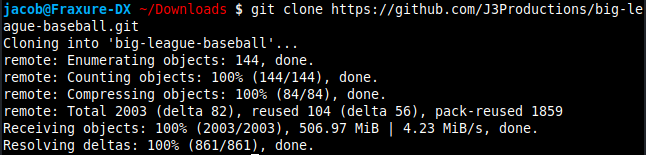
\includegraphics[width=1\linewidth]{umInclude/clone}
\end{center}
This will download the game to your computer just like that! However, if you do not have Git installed, you can still download BIG LEAGUE BASEBALL on the game's GitHub page.\\
Open up your preferred web browser (Chrome, Firefox, Midori, etc.) and navigate to\linebreak \href{https://github.com/J3Productions/big-league-baseball}{\texttt{github.com/J3Productions/big-league-baseball}}. There, you will find the game's GitHub page (we're open source, you're welcome to fork!).
\begin{center}
	
\includegraphics[width=1\linewidth]{umInclude/github}
\end{center}
From there, you will see a green button labeled ``Clone or download.'' Click on the button, and then click on the button labeled ``Download ZIP.''
\begin{center}
	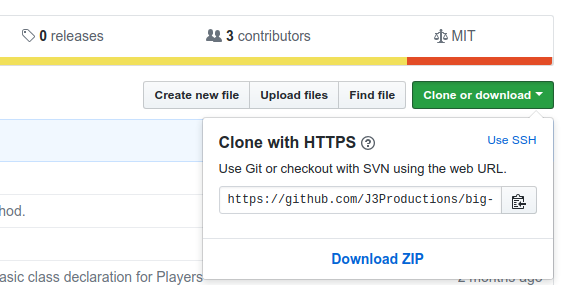
\includegraphics[width=0.75\linewidth]{umInclude/download}
\end{center}
This will download the game a compressed ZIP file to your computer. Extract the file with your preferred archive manager, and you have BIG LEAGUE BASEBALL downloaded!

\section{Installing}
Now that you have the BIG LEAGUE BASEBALL downloaded, the game must be installed (well, not technically, since the game just needs to download a few dependencies, but nothing actually gets installed to your computer). Let's get started!\\
Enter the directory of your downloaded game, and open a terminal. From there, type and execute the command:
\begin{displayquote}
	\texttt{npm install --production}
\end{displayquote}
\begin{center}
	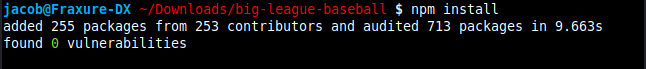
\includegraphics[width=1\linewidth]{umInclude/install}
\end{center}
This will pull all of the required dependencies for playing the game in from the internet. You are now ready to start the game up!\\
\textit{NOTE: If you are unable to use the \texttt{npm} command, you may need to install Node.js: \url{https://nodejs.org}}

\section{Starting the Game}

Now that the game is downloaded and so are all the dependencies, it's time to start up BIG LEAGUE BASEBALL!\\
From the same directory that you ran \texttt{npm install} from, run the following command:
\begin{displayquote}
	\texttt{npm run test}
\end{displayquote}
Once you have done this, open your favorite web browser (Chrome, Firefox, Vivaldi, etc.) and navigate to \href{http://localhost:3000}{\texttt{localhost:3000}}. There, the game should be up and waiting for you to play!

\chapter{Playing the Game}
\begin{center}
	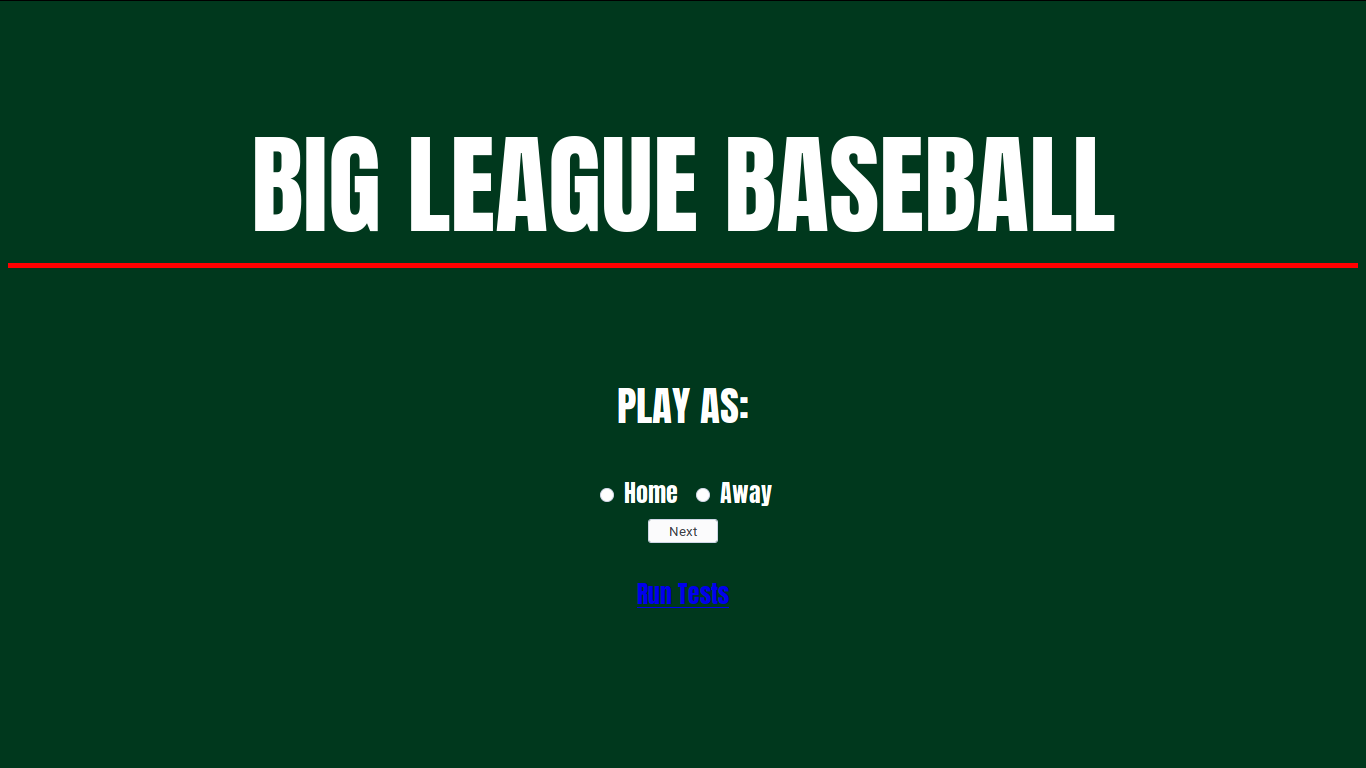
\includegraphics[width=1\linewidth]{umInclude/start}
\end{center}
Congratulations, if you're seeing this screen right now, then you've followed all of the instructions properly and nothing went wrong, so you're ready to play some BIG LEAGUE BASEBALL! Let's get started, shall we?

\section{The Title Screen}
On the title screen, you'll see two options for who to play as: Home and Away. In case you've forgotten, the Away team bats in the top of the inning, and the Home team bats in the bottom of the inning. So if you'd like to be the first to bat, choose Away. If you'd like to be the first to pitch, choose Home.\\
But remember, if the game goes to extra innings and you go ahead as the Away team, the Home team still has a chance to win the game in the bottom half of the inning, whereas if you go ahead as the Home team, that's the game.\\
You will also see a link labeled ``Run Tests'' on the title screen. If you click this link, you will be taken to the game's self-testing software that makes sure everything in the game is working to perfection just for you (to see the results, open the browser console by pressing F12 on the test page).

\section{The Interface}
\begin{center}
	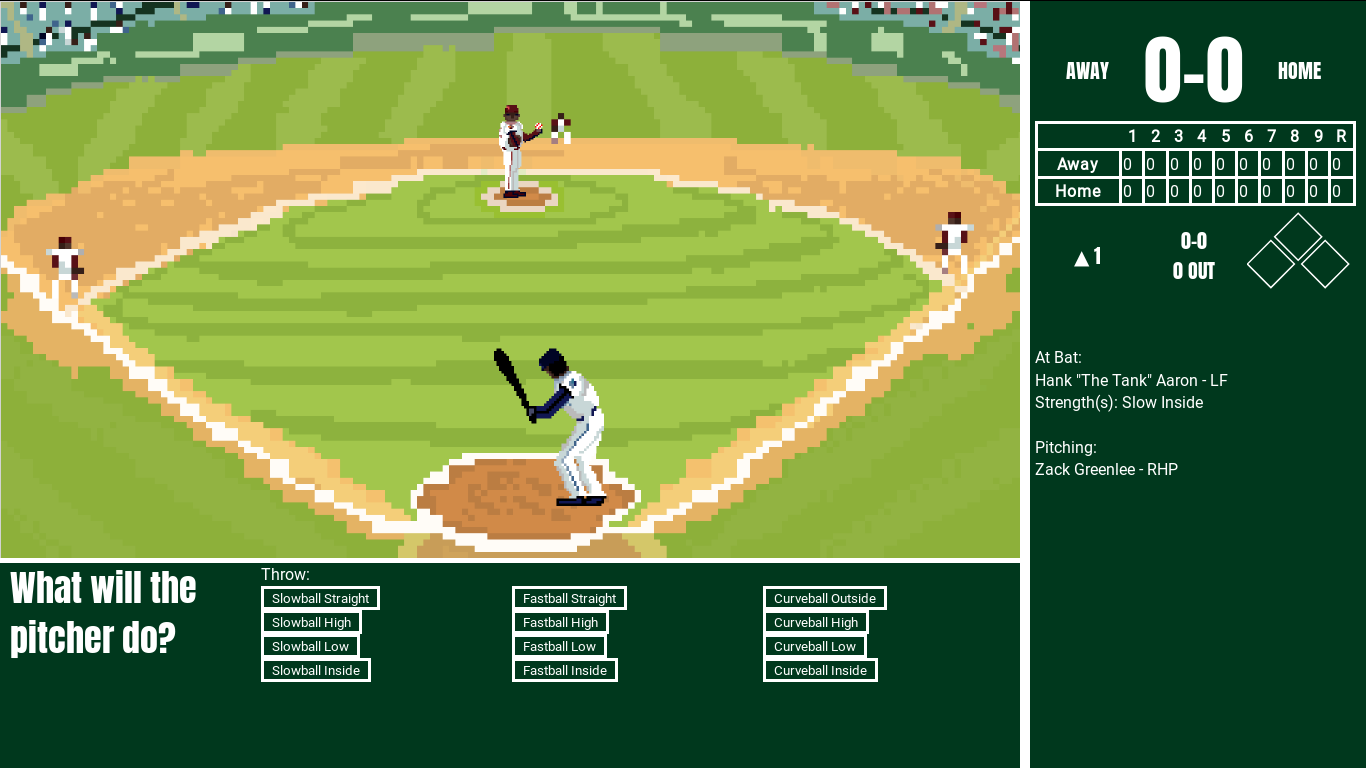
\includegraphics[width=1\linewidth]{umInclude/interface}
\end{center}
Once you've selected your side and click ``Next,'' you'll be taken to the game! Ah, there's nothing like a day out at the ballpark! But before we get started playing, you'll need to know what the different parts of the game display are and what they do.

\subsection{The Animation Area}
\begin{center}
	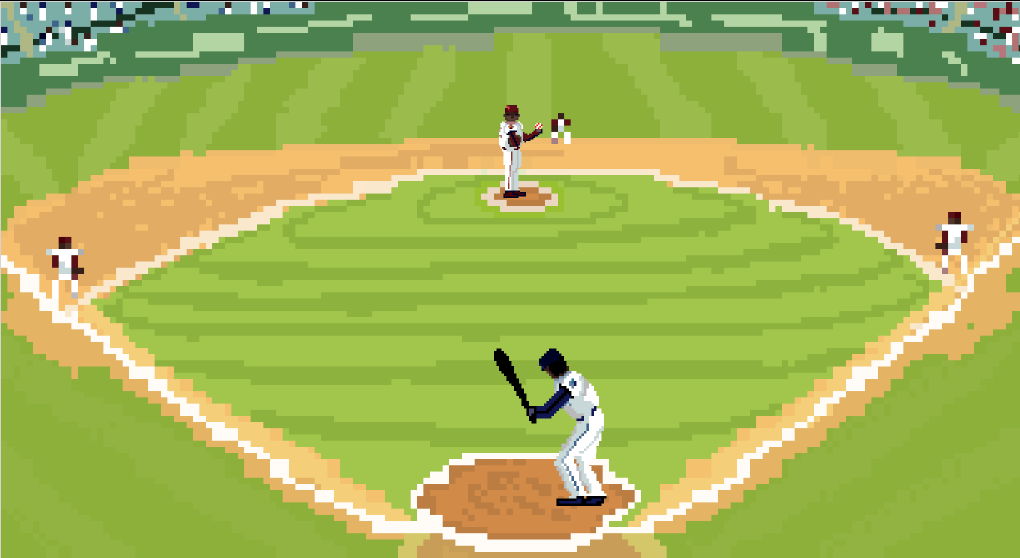
\includegraphics[width=1\linewidth]{umInclude/animation}
\end{center}
Here's where you'll see all of your actions acted out and see the result of each pitch. Select your moves wisely, or else this display could quickly become a tragedy for your team!

\subsection{The Score Area}

\begin{wrapfigure}{R}{0.3\linewidth}
	\begin{center}
		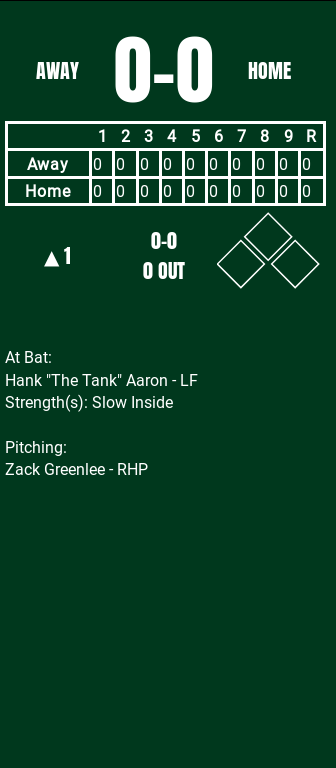
\includegraphics[width=1\linewidth]{umInclude/score}
	\end{center}
\end{wrapfigure}
This is where your score and all other important game-related stuff is located. Here's what it all means:\\
\begin{itemize}
	\item The element on the very top displays the game's score, with the Away team's score on the left and the Home team's score on the right. Whoever has more runs at the end of 9 innings is the winner, simple as that!
	\item The second element shows the score again, but it displays the number of runs scored in each inning. Awesome!
	\item Below that on the left is the current inning. $ \Delta $ denotes the top of the inning while $ \nabla $ denotes the bottom of the inning.
	\item In the middle is the batter's count - balls and then strikes, as well as the number of outs.
	\item On the right is what the bases look like. If a base is clear, there is nobody on that base, but if it is yellow, then there is a man on that base.
	\item Below all of that shows you who is currently pitching and who is at bat, as well as what their batting strengths are.
\end{itemize}

\subsection{The Message/Decision Area}
\begin{center}
	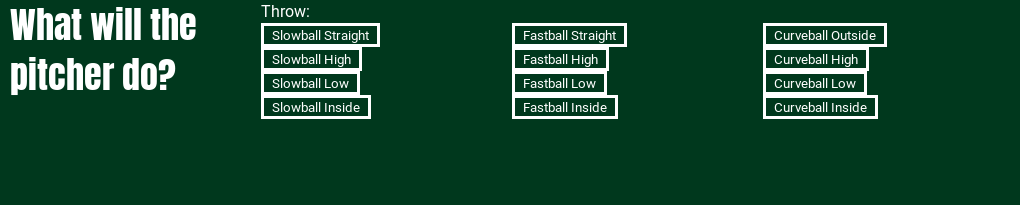
\includegraphics[width=1\linewidth]{umInclude/message}
\end{center}
This is where you'll decide what to do and where you'll see the results of your action. If your team is currently pitching, you'll see the pitches that your pitcher can throw, but if your team is currently batting, you'll see the pitches that your batter can swing for. After you select an action, the play will occur, and this area will describe the result to you.

\section{Batting}
Alright, you know all the ins and outs of the interface now and probably feel like you could manage an actual big-league team (I hear the Orioles are looking for a new manager). It's time to start playing! If you're up to bat (in the top of the inning for the Away team and the bottom of the inning for the Home team), here's what your Decision Area will look like:
\begin{center}
	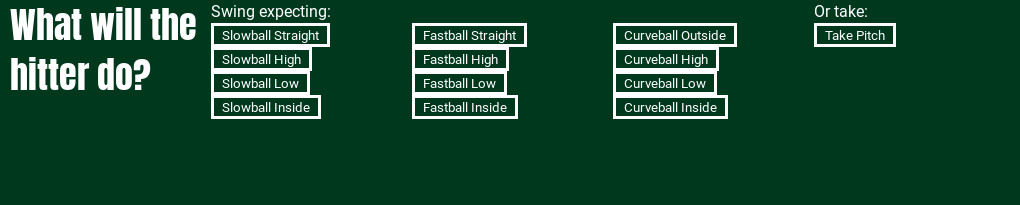
\includegraphics[width=1\linewidth]{umInclude/hitter}
\end{center}
Your objective is to try to figure out what the pitcher might throw you and try to swing for that pitch. For example, you might expect the pitcher to throw you a straight fastball, so you might select ``Fastball Straight.'' Or, you might choose to not swing at all if you expect that the pitcher will throw you a ball. To do this, select ``Take Pitch.''\\
The pitcher will try to throw you strikes when they expect you to take, and he will try to throw you balls when they expect you to swing, so swing strategically!\\
One more thing, you may have noticed in the Score area that every batter has certain pitches that are his strengths. In the major leagues, batting strengths and weaknesses of players are generally known to their opponents. Pitchers try to avoid pitching to the batter's strength, but occasionally, a pitcher may try to cross up a batter and pitch to his strength when he thinks the batter may be looking for something else.\\
If a player throws the batter one of his strengths, and he swings expecting that strength, the batter will automatically hit the ball better and have a greater chance for a safe hit.

\section{Pitching}
So now your team is out on the field and the game is in the hands of your pitcher. You'll get your chance to pitch in the top of the inning if you're the Home team and in the bottom of the inning if you're the Away team. Here's what your Decision Area will look like:
\begin{center}
	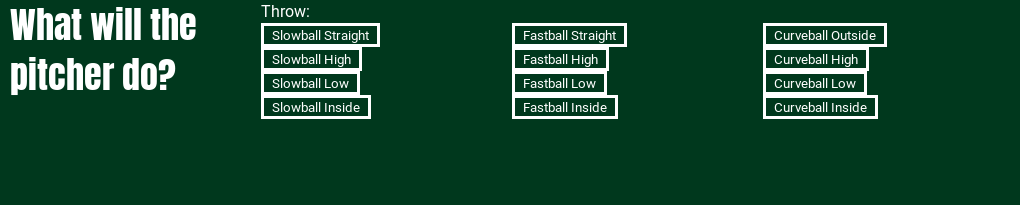
\includegraphics[width=1\linewidth]{umInclude/message}
\end{center}
Your job is to make sure that the batter doesn't get on base by throwing them pitches strategically. Straight, inside, and outside pitches will be counted as strikes if the batter takes, and high and low pitches will be counted as balls if the batter takes. However, if the batter swings for a pitch that would be a strike, there is a better chance that they will get a hit out of it, and if the batter swings for a pitch that would be a ball, there is a better chance that they will swing and miss on it. So try to guess when the batter will swing and when he will take!\\
And remember, 3 strikes = 1 out, 4 balls = 1 walk to put a man on base, and 3 outs = the end of the inning.

\section{Winning the Game}
The game will end if one of the following happens:
\begin{itemize}
	\item The Home team has more runs than the Away team after the top of the 9th inning.
	\item The Away team has more runs than the Home team after the bottom of the 9th inning or later.
	\item The Home team scores enough runs to take the lead in the bottom of the 9th inning or later (resulting in a walk-off, as you might call it).
\end{itemize}
But how do you score runs? Either by hitting the ball out of the park, or by chaining hits together. How do you do that? And if you're the pitcher, how do you prevent the other team from doing that? So here are a few tips for both sides.\\\\
For the pitcher:
\begin{enumerate}
	\item Use pitches out of the strike zone as often as possible (the batter has less chance for a safe hit with these pitches).
	\item Mix up your pitches so the batter will swing at pitches out of the strike zone
	\item If the batter sees too many bad pitches out of the strike zone, he will start taking, and this may add up to walking the batter.
	\item Cross up the batter occasionally by throwing one of his strengths when he isn't looking for it.
\end{enumerate}
For the batter:
\begin{enumerate}
	\item Don't swing at every pitch. Wait for a good one (a pitch in the strike zone).
	\item Swinging in the strike zone gives you the best chance for a safe hit. You won't hit the ball squarely and may miss it entirely if you swing out of the strike zone.
	\item If your strength is out of the strike zone, occasionally swing at it.
	\item Watch the ball and strike count.
\end{enumerate}
For both batter and pitcher, remember that all high and low pitches are out of the strike zone and that straight, inside, and outside pitches are in the strike zone.

\chapter{Acknowledgements}

Here's the people who made this game possible:\\

3M Games - Original Author of BIG LEAGUE BASEBALL, Portions of this manual were taken from the original game's manual\\

Jielong Cong - Animator and Graphic Designer\\

Darrell Parnell - Person who Introduced Jacob to BIG LEAGUE BASEBALL, and who Jacob Borrowed a Copy of the Game From while Developing this Game\\

Jacob Parnell - UI and Game Logic Programmer, Had Idea to Make Game\\

Jason Purinton - Audio Engineer, Base Game Programmer\\

\bigskip\bigskip\bigskip\bigskip\bigskip\bigskip\bigskip\bigskip\bigskip\bigskip\bigskip\bigskip\bigskip\bigskip\bigskip\bigskip\bigskip\bigskip\bigskip\bigskip\bigskip\bigskip\bigskip\bigskip\bigskip\bigskip
Copyright 1967, 2018 3M Co., J3 Productions

\end{document}          
